%% LaTeX Beamer presentation template (requires beamer package)
%% see http://latex-beamer.sourceforge.net/
%% idea contributed by H. Turgut Uyar
%% template based on a template by Till Tantau
%% this template is still evolving - it might differ in future releases!

\documentclass{beamer}
\usepackage{graphicx}
\mode<presentation>
{
\usetheme{Frankfurt}

\setbeamercovered{transparent}
}

\usepackage[english]{babel}
\usepackage[latin1]{inputenc}

% font definitions, try \usepackage{ae} instead of the following
% three lines if you don't like this look
\usepackage{mathptmx}
\usepackage[scaled=.90]{helvet}
\usepackage{courier}


\usepackage[T1]{fontenc}
\usepackage{xcolor}
\usepackage{tikz}
\usepackage{multimedia}
\usepackage{setspace}
\usepackage{eurosym}
\usepackage{verbatim}

\usetikzlibrary{arrows,shapes,positioning}
\usetikzlibrary{shapes.arrows}
\usetikzlibrary{shadows}
\usetikzlibrary{calc}
\usetikzlibrary{decorations.pathreplacing}
\usetikzlibrary{decorations.pathmorphing}
\usetikzlibrary{decorations.markings}

\tikzstyle{block}=[draw opacity=0.7,line width=1.4cm]

\useinnertheme{rounded}


\setlength{\fboxrule}{2pt}

% For every picture that defines or uses external nodes, you'll have to
% apply the 'remember picture' style. To avoid some typing, we'll apply
% the style to all pictures.







\title{What is CFS++?}

%\subtitle{}

% - Use the \inst{?} command only if the authors have different
%   affiliation.
%\author{F.~Author\inst{1} \and S.~Another\inst{2}}
\author{Fabian Wein}

% - Use the \inst command only if there are several affiliations.
% - Keep it simple, no one is interested in your street address.
% \institute[Universities of]
% {
% \inst{1}%
% Department of Computer Science\\
% Univ of S
% \and
% \inst{2}%
% Department of Theoretical Philosophy\\
% Univ of E}

%\date{Date / Occasion}


% This is only inserted into the PDF information catalog. Can be left
% out.
\subject{Talks}



% If you have a file called "university-logo-filename.xxx", where xxx
% is a graphic format that can be processed by latex or pdflatex,
% resp., then you can add a logo as follows:

% \pgfdeclareimage[height=0.5cm]{university-logo}{university-logo-filename}
% \logo{\pgfuseimage{university-logo}}



% If you wish to uncover everything in a step-wise fashion, uncomment
% the following command:

%\beamerdefaultoverlayspecification{<+->}

\begin{document}

\tikzstyle{every picture}+=[remember picture]
\tikzstyle{every node}+=[drop shadow,rounded corners=1mm]


\begin{frame}
\titlepage
\end{frame}

\begin{frame}
\frametitle{Outline}
\tableofcontents
% You might wish to add the option [pausesections]
\end{frame}


\section{Introduction}

\subsection{Boundary Conditions}

\begin{frame}
\frametitle{Boundary Conditions}

Here we do \textbf{NOT} talk about 
\begin{itemize}
  \item Features of CFS++
  \item How to use CFS++
  \item How to develop CFS++
\end{itemize}
This is also \textbf{NO} \ldots
\begin{itemize}
  \item marketing talk about how great CFS++ is
  \item how CFS++ can contribute to universal peace!
\end{itemize}

\end{frame}


\begin{frame}
\frametitle{What is CFS++?}
\begin{itemize}
  \item FEM implementation in CFS
  \begin{itemize}
    \item \textbf{C}oupled \textbf{F}ield \textbf{S}imulation
    \item Topology optimization
  \end{itemize}  
  \item Academic Software
    \begin{itemize}
      \item Students/ M.Sc./ Ph.D. students use it 
      \item M.Sc./ Ph.D. students develop it
    \end{itemize}  
  \item Goes back to Manfred Kaltenbacher
    \begin{itemize}
    \item Previous versions in Matlab and Fortran 
  \end{itemize}  
  \item A commercial fork is NACS by Simetris 
\end{itemize}
\end{frame}

\subsection{History}
\begin{frame}
\frametitle{History}

Genesis
\begin{itemize}
  \item Start 2002 at LSE
  \item Group of Manfred Kaltenbacher
  \item Since then ca. 5-8 developers 
\end{itemize}

Optimization
\begin{itemize}
  \item Inverse piezo identification by Tom Lahmer but no framework
  \item Since 2006 structural optimization framework

\end{itemize}

Diversity
\begin{itemize}
  \item 2002 LSE ``Sensor-Technology''
  \item 2008 Klagenfurt ``Applied Mechatronics'': Manfred Kaltenbacher
  \item 2009 AM2 ``Applied Mathemathics II'': Group Michael Stingl 
\end{itemize}
\end{frame}

\begin{frame}
\frametitle{Commerical Fork NACS}

SIMetris GmbH - spinoff of LSE 2006
\begin{itemize}
 \item Martin Meiler and Herman Landes
 \item Product NACS is based on CFS++
 \item Handle simulation projects
\end{itemize}

NACS
\begin{itemize}
  \item CFS developers work for SIMetris
  \item Linux and Windows
  \item Integrated user interface
  \item No optimization
  \item No merges between CFS and NACS!
  \item Professional and student license available
  \item Support available
\end{itemize}

\end{frame}


\begin{frame}
\frametitle{Legal State of CFS++}
Overview
\begin{itemize}
  \item Master mind/ ``owner'' is Manfred Kaltenbacher
  \item No license file exists!
  \item CFS++ is considered open source as it is based on public fundings
\end{itemize}

Gentleman's agreement
\begin{itemize}
  \item CFS++ shall \textbf{not} be publicly available
  \item Manfred Kaltenbacher is informed prior to distribution
  \item IMHO: NACS should be used for commercial use (Fabian Wein)
\end{itemize} 
\end{frame}

\section{Structure}

\subsection{Structure}

\begin{frame}
\frametitle{Focus of CFS++}
Multi purpose vehicle
\begin{itemize}
  \item Simulation tool for engineers
  \item Research code
  \item Academic optimization tool
\end{itemize}
Focus on engineering problems
\begin{itemize}
  \item CFS++ is an application and not a library
  \item Solves physical problems
  \item No arbitrary mathematical constructs
\end{itemize}
\end{frame}

\begin{frame}
\frametitle{Schema}
\begin{center}
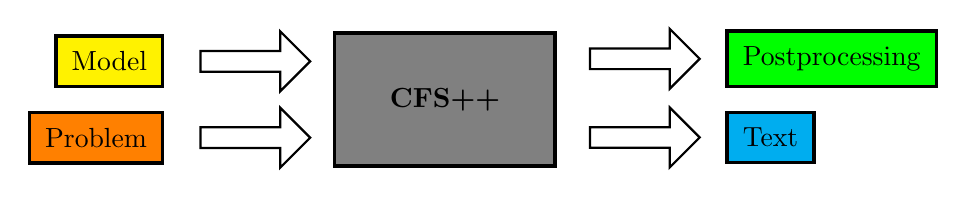
\begin{tikzpicture}[draw=black,every shadow/.style={opacity=0.0},very thick, node distance=2mm,
  shorten >= 2mm, shorten <= 1mm, scale = 0.99]
  \node[draw, fill=gray, inner sep=7mm] (center) { \textbf{CFS++} };

  \node[above left=of center.west,draw, fill=yellow, inner sep=2mm,xshift=-20mm] (left) { Model };
  \node[below left=of center.west,draw, fill=orange, inner sep=2mm,xshift=-20mm] (leftdown) { Problem };
  \node[above right=of center.east,draw, fill=green, inner sep=2mm,xshift=20mm] (right) { Postprocessing };
  \node[below right=of center.east,draw, fill= cyan, inner sep=2mm,xshift=20mm] (rightdown) { Text };

  \path (left.east) -- node[midway,single arrow,thick,draw=black,text width=10mm] {} ++(22mm,0);
  \path (leftdown.east) -- node[midway,single arrow,thick,draw=black,text width=10mm] {} ++(22mm,0);

  \path (right.west) -- node[midway,single arrow,thick,draw=black,text width=10mm] {} ++(-22mm,0);
  \path (rightdown.west) -- node[midway,single arrow,thick,draw=black,text width=10mm] {} ++(-22mm,0);
\end{tikzpicture}
\end{center}

\begin{itemize}
  \item \textbf{Model:} mesh data
  \item \textbf{Problem:} XML file defining problem and physical properties
  \item \textbf{CFS++:} command line based FEM solver/ optimizer
  \item \textbf{Postprocessing:} visualization and calculations
  \item \textbf{Text:} detailed information in XML format
\end{itemize}
\end{frame}

\begin{frame}
\frametitle{Model (Preprocessing)}
Mesh
\begin{itemize}
  \item all dimensions, mixed
  \item all type of primitives, mixed
  \item structure by ``regions'' and ``named elements''
\end{itemize}
Preprocessing
\begin{itemize}
  \item GiD
  \begin{itemize}
    \item interactive visual modeling 
    \item TCL based scripting (CFS++ plugin)
    \item $\approx$ 150\,\euro
  \end{itemize}
  \item ANSYS
  \begin{itemize}
    \item legacy Prep7
    \item for sophisticated geometries
  \end{itemize}
  \item Generic mesh creation   
\end{itemize}
\end{frame}

\begin{frame}[containsverbatim]
\frametitle{Problem XML File}
Example (fragment)
\footnotesize\begin{verbatim}
   <pdeList>
      <mechanic subType="planeStrain">
        <regionList>
          <region name="mech"/>
        </regionList>
        <bcsAndLoads>
          <dirichletHom name="flexible" dof="y"/>
          <load name="load" dof="y" value="-1e0"/>
        </bcsAndLoads>
\end{verbatim}
\normalsize
XML-Schema definition
\begin{itemize}
  \item Defined syntax and default values
  \item Editors with content assistant 
\end{itemize}
\end{frame}

\begin{frame}
\frametitle{CFS++ Features}
Physics (almost arbitrary coupled)
\begin{itemize}
  \item Linear and nonlinear elasiticity
  \item Linear and nonlinear piezoelectricity
  \item Linear and nonlinear acoustics
  \item Magnetics
  \item Electrostatic
  \item Navier-Stokes
\end{itemize}
Optimization
\begin{itemize}
  \item SIMP (elasticity, piezoelectricity)
  \item Inverse homogenization
  \item Parametric shape-optimization
  \item Level-set and topology gradient (partially)
\end{itemize}
\end{frame}

\begin{frame}
\frametitle{CFS++ Features cont.}

Solvers (linear system)
\begin{itemize}
  \item Pardiso (direct and iterative)
  \item ILUPACK (iterative)
  \item CHOLMOD
  \item Standard: PCG, GMRES, LDL
\end{itemize}
Solvers (optimizers)
\begin{itemize}
  \item SCPIP (MMA)
  \item SnOpt
  \item IPOPT
  \item Optimality condition
\end{itemize}
Missing
\begin{itemize}
  \item Adaptive mesh refinement
  \item Adaptive time stepping
\end{itemize}
\end{frame}


\begin{frame}
\frametitle{Output}
Visual postprocessing
\begin{itemize}
  \item GiD
  \item Paraview (by CFS++ HDF5 reader plugin)
  \item GMV
\end{itemize}
Numerical postprocessing
\begin{itemize}
  \item HDF5 binary format by C and Matlab API
  \item Textdata
\end{itemize}
User feedback
\begin{itemize}
  \item Structured XML file

\end{itemize}
\end{frame}



\section{Development}

\subsection{Developers}

\begin{frame}
\frametitle{Type of Developers}
Heros
\begin{itemize}
  \item Altruistic feature contribution and refactoring
  \item \textbf{Andreas Hauck} \ldots
\end{itemize}
Contributers
\begin{itemize}
  \item Contribute research code to CFS++
  \item Fix and clean common code and documentation
\end{itemize}
Rookies
\begin{itemize}
  \item Contribute their features by copy \& paste
  \item Require later refactoring by heros  
\end{itemize}

\end{frame}


\begin{frame}
\frametitle{Version Control}
\begin{minipage}{0.65\textwidth}
\begin{itemize}
  \item Common software with common features
  \item Everybody works on own branches
  \item Test cases prevent side effects
  \item Not everything ends on the trunk
\end{itemize}
\end{minipage}
\begin{minipage}{0.3\textwidth}
  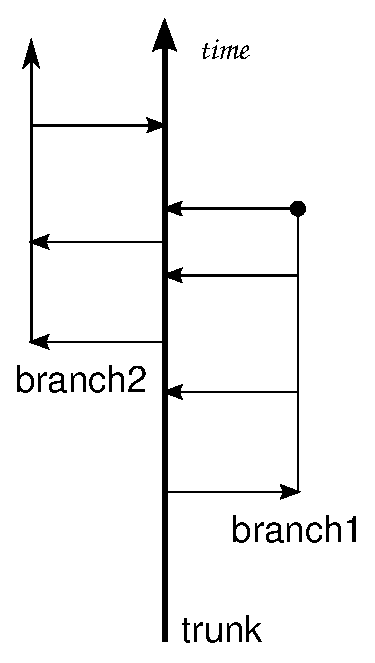
\includegraphics[width=0.9\textwidth]{branching}
\end{minipage}
\end{frame}

\begin{frame}
\frametitle{Development process}
\begin{itemize}
  \item Collaborative development
  \item No relase management 
  \item Shared code ownership $\to$ code cleanup be heros
  \item Significant changes are discussed
  \begin{itemize}
    \item monthly mensa meetings LSE/AM2
    \item skype discussions with Klagenfurt
    \item CFS++ developer meetings planned
  \end{itemize}
\end{itemize}
Pros
\begin{itemize}
  \item Features and bug fixes ``for free''
  \item Extends lifetime of own code
\end{itemize}
Cons
\begin{itemize}
  \item Complex code base, no rapid prototyping
  \item Test cases are necessary 
\end{itemize}
\end{frame}

\section{Using CFS++}
\subsection{Learning CFS++}

\begin{frame}
\frametitle{Learning CFS - the classical way}
Theory
\begin{itemize}
  \item Lecture ``CAE of Sensors and Actuators''
  \item Lecture ``Numerical Simulation of Electromechanical Transducers''
  \item Based on \textit{M. Kaltenbacher; Numerical Simulation of Mechatronic Sensors and Actuators; Springer; 2007}
  \begin{itemize}
    \item most features of CFS are found in the book
    \item common notation
  \end{itemize}  
\end{itemize}
Usage of CFS++
\begin{itemize}
  \item Tutorials to the lectures
  \item Didactic set of homework and project tasks
  \item User manual for students 
\end{itemize}
\end{frame}

\end{document}
